\documentclass{article}
\usepackage[hyphens]{url}
\usepackage{mathtools}
\usepackage{amsmath}
\usepackage{listings}
\usepackage{graphicx}
\usepackage[margin=1in]{geometry}
\usepackage{float}
\floatstyle{boxed}
\restylefloat{figure}
\lstset{breaklines=true}
\begin{document}


\title{CS595 Intro to Web Science, Assignment \#7}
\author{Valentina Neblitt-Jones}
\date{November 7, 2013}
\maketitle



\section*{Question 1}

Using D3, create a graph of the Karate club before and after the split \\

Weight the edges with data from: \url{http://vlado.fmf.uni-lj.si/pub/networks/data/ucinet/zachary.dat} \\

Have the transition from before/after the split occur on a mouse click.  \\

%\begin{itemize}
%\item 
%\item
%\end{itemize}

\subsection*{Answer to Question 1}


%\begin{figure}[H]
%\centering
%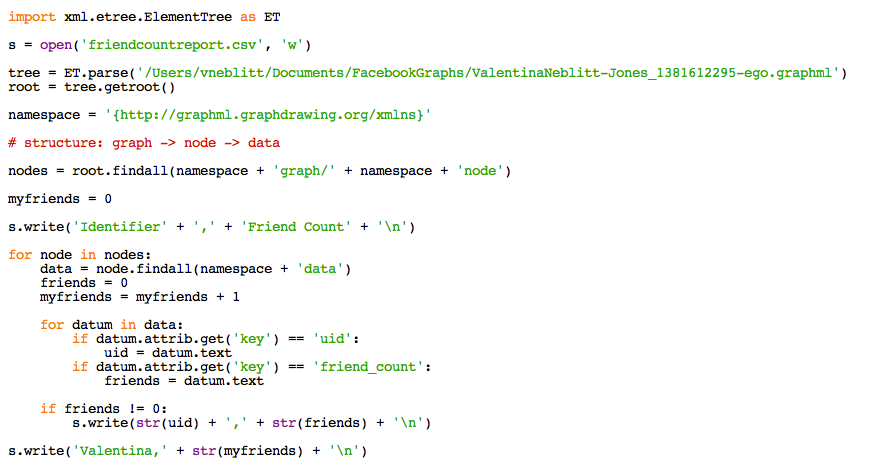
\includegraphics[scale=0.50]{q1/GetFriendCountsCode}
%\caption{Showing Friend Count}
%\label{GetFriendCountsCode}
%\end{figure}

%\begin{table}[!h]
%\centering

%\begin{tabular}{c c c c}
%\hline
%Identifier & Model &  Actual & Hit/Miss \\
%\hline
%\hline
%1 & Mr. Hi & Mr. Hi & Hit \\
%2 & Mr. Hi & Mr. Hi & Hit \\
%3 & Mr. Hi & Mr. Hi & Hit \\
%4 & Mr. Hi & Mr. Hi & Hit \\
%5 & Mr. Hi & Mr. Hi & Hit \\
%6 & Mr. Hi & Mr. Hi & Hit \\
%7 & Mr. Hi & Mr. Hi & Hit \\
%8 & Mr. Hi & Mr. Hi & Hit \\
%9 & Mr. Hi & Mr. Hi & Hit \\
%10 & Mr. Hi & John & Miss \\
%\hline
%\end{tabular}
%\caption{Results of Model vs. Actual}
%\end{table}

\newpage

\section*{Extra Credit, 3 Points}

Use D3 to create a who-follows-whom graph of your Twitter account. Use my Twitter account (phonedude\_mln) if you do not have an interesting number of followers.

%\begin{table}[!h]
%\centering
%\caption{Results of Model vs. Actual}
%\begin{tabular}{c c c c}
%\hline
%Identifier & Model &  Actual & Hit/Miss \\
%\hline
%\hline
%0.150 & 0.014 & Mr. Hi & Hit \\
%0.085 & John & Mr. Hi & Hit \\
%\hline
%\end{tabular}
%\end{table}

\subsection*{Answer to Extra Credit}





\newpage

\section*{Resources}

\begin{itemize}
\item Csardi, Gabor. Network Analysis with igraph. \url{http://igraph.sourceforge.net/igraphbook/index.html}
\item Poulson, Barton. R Statistics Essential Training. \url{http://www.lynda.com/course20/R-tutorials/R-Statistics-Essential-Training/142447-2.html}
\item Rice, Ken \& Lumley Thomas. Writing Loops. \url{http://faculty.washington.edu/kenrice/sisg/SISG-08-05.pdf}
\item Sourceforge.net. Network Analysis and Visualization. \url{http://igraph.sourceforge.net/doc/R/00Index.html}
\item Stack Overflow. Are there implentations of algorithms for community detection in graphs? \url{http://stackoverflow.com/questions/5822265/are-there-implementations-of-algorithms-for-community-detection-in-graphs}
\item Stack Overflow. What are the differences between community detection algorithms in igraph? \url{http://stackoverflow.com/questions/9471906/what-are-the-differences-between-community-detection-algorithms-in-igraph/9478989#9478989}
\item Zachary, Wayne. An Information Flow Model for Conflict and Fission in Small Groups. \url{http://aris.ss.uci.edu/~lin/76.pdf}


\end{itemize}

\end{document}